\chapter{Microservizio EventExport}
\label{cap:MicroservizioEventExport}

\section{Panoramica del microservizio}
\label{sec:ScopoDelMicroservizio}
Lo scopo del microservizio \textit{EventExport} è quello di elaborare dei \textbf{Business Event}, che arrivano dal microservizio \textit{EventEngine} 
(sezione \ref{subsubsec:event_engine}) e di comunicarli al cliente.\\\\
\textbf{EventExport} è configurabile in maniera differente per ogni cliente, di modo che ad un cliente vengano inviati solo alcuni tipi di eventi.
Ad esempio, un cliente potrebbe essere interessato solo agli eventi di creazione di un ordine, mentre un altro potrebbe voler ricevere tutti gli aggiornamenti
riguardo alla posizione dell'ordine da lui effettuato.
Questa configurazione è gestita tramite una tabella \textit{LogicDeterminationEvent} che contiene le regole di filtro per ogni cliente.
\begin{figure}[htbp]
    \centering
    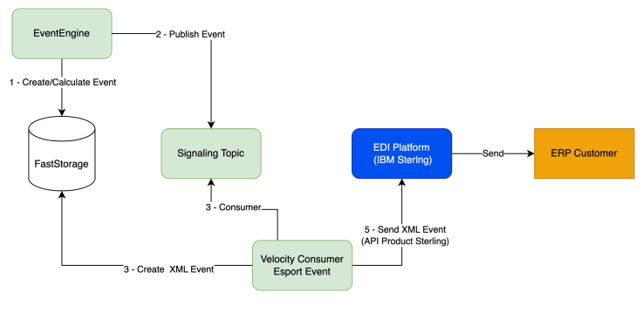
\includegraphics[width=\textwidth]{images/EventExport/EventExport_architecture.png}
    \caption{architettura con il microservizio \textit{EventExport}}
    \label{fig:EventExport_architecture}
\end{figure}\\
Il microservizio compie le seguenti operazioni:
\begin{enumerate}
    \item Consumare il \textit{Signaling Topic} (topic Kafka) applicando un filtro basato su una tabella di configurazione.
    \item Controllare se l'evento deve essere inviato. Non è necessario inviare eventi già inviati a meno di modifiche su campi significati 
    (anche questi definiti in base alla configurazione).
    \item Creare un file XML con i dati richiesti dal cliente. I dati sono definiti in base a dei template che vengono compilati in base alla configurazione.
    \item Inviare il file XML ad un altro servizio che si occuperà di inviare al cliente una mail.
    \item Loggare l'evento, compreso di XML, in una tabella (\textit{TransportOrdersExportEvents}) per tenere traccia degli eventi inviati.
\end{enumerate}


\section{Lettura del Signaling Topic}
\label{sec:LetturaDelSignalingTopic}
La lettura del \textit{Signaling Topic} avviene tramite un \textit{Consumer} Kafka.
Flink mette a disposizione un \textit{Kafka Consumer} 
che permette agevolmente di leggere i messaggi da un topic Kafka: \texttt{org.apache.flink.connector.kafka.source.KafkaSource}
Il \textit{Broker} Kafka su cui vive il \textit{Signaling Topic} è configurato per usare un sistema di autenticazione basato su \textit{SASL/SSL},
inoltre gli eventi sul topic sono serializzati tramite \textit{Apache Avro} (sezione \ref{subsec:avro_overview}) quindi è necessario configurare il \textit{Consumer Kafka} di conseguenza.
\begin{code}
    \inputminted[linenos]{java}{listings/EventsExport/KafkaSources.java}
    \caption{Configurazione del Kafka Consumer}
    \label{lst:KafkaSources}
\end{code}
Come mostrato nel codice \ref{lst:KafkaSources}, il \textit{Consumer Kafka} è configurato per leggere i messaggi dal topic \textit{Signaling Topic} 
ed il deserializzatore utilizzato è\\ \texttt{org.apache.flink.api.common.serialization.DeserializationSchema},
una classe messa a disposizione da Flink per deserializzare i messaggi \textit{Avro}.
Le righe 15,18,19 e 26 sono tipiche di un \textit{Consumer Kafka} scritto con \textit{Flink}, è presente infatti la creazione del \textit{builder} (riga 15),
la definizione del \textit{topic} da cui leggere (riga 18), l'offset da cui iniziare a leggere (riga 19) e  la creazione del \textit{Consumer} (riga 26).
Invece nelle righe 16 e 20-21 si possono leggere rispettivamente la configurazione del \textit{Kafka Consumer} e la configurazione del deserializzatore \textit{Avro}.\\\\
Nella chiamata alla funzione \texttt{forSpecific} a riga 21 i parametri sono la classe in cui verrà deserializzato il messaggio, l'url dello \textit{Schema Registry}
e le properties contenenti credenziali per accedere allo \textit{Schema Registry}. 
La configurazione del \textit{Kafka Consumer} e del deserializzatore \textit{Avro} è definita in un file \textit{.properties} e principalmente contiene
l'url dell'endpoint, le credenziali e diversi parametri per la connessione.
In un caso (\textit{Kafka}) è riferita al \textit{Broker Kafka} e nell'altro allo \textit{Schema Registry} (\textit{Avro}).

\section{Lettura della tabella di configurazione}
\label{sec:LetturaDellaTabellaDiConfigurazione}
La tabella di configurazione è una tabella \textit{SQL} chiamata \textit{LogicDeterminationEvent} e contiene le regole di filtro per ogni cliente.
La connessione al database è gestita tramite \textit{JPA} e la libreria \textit{Hibernate} (sezione \ref{subsec:hibernate_overview}) con un sistema di caching
per evitare richieste ripetute al database. La cache viene aggiornata ogni ora.
\begin{figure}[htbp]
    \centering
    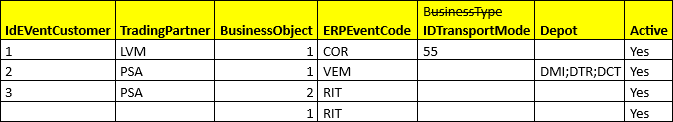
\includegraphics[width=\textwidth]{images/EventExport/LogicDeterminationEvent.png}
    \caption{Tabella \textit{LogicDeterminationEvent}}
    \label{fig:LogicDeterminationEvent}
\end{figure}
